\documentclass[11pt,spanish]{beamer}
\usepackage{mathpazo}
\usepackage{tgheros}
\renewcommand{\familydefault}{\sfdefault}
\usepackage[T1]{fontenc}
\usepackage[utf8]{inputenc}
\usepackage{babel}
\usepackage{amsmath}
\usepackage{amssymb}
\usepackage{array}
\usepackage{graphicx}
\usepackage{tikz}
\usetikzlibrary{arrows.meta,automata,calc,positioning,shapes.geometric}
\usepackage{listings}

\definecolor{Guinda}{rgb}{0.49,0.05,0.12}
\definecolor{Rojo}{rgb}{0.8,0,0}
\definecolor{indiagreen}{rgb}{0.07,0.53,0.03}
\definecolor{anti-flashwhite}{rgb}{0.95,0.95,0.96}
\definecolor{pastelblue}{rgb}{0.78,0.87,0.96}
\definecolor{pastelgreen}{rgb}{0.82,0.92,0.78}
\definecolor{pastelpeach}{rgb}{0.98,0.84,0.72}
\definecolor{pastelrose}{rgb}{0.96,0.78,0.84}
\definecolor{pastelviolet}{rgb}{0.86,0.80,0.96}
\definecolor{pastelyellow}{rgb}{0.98,0.93,0.70}

\usecolortheme[named=indiagreen]{structure}
\usetheme{Boadilla}
\usefonttheme{structurebold}
\setbeamertemplate{itemize items}[default]
\setbeamertemplate{enumerate items}[default]
\setbeamertemplate{navigation symbols}{}
\setbeamercolor{block title}{fg=white,bg=indiagreen!85!black}
\setbeamercolor{block body}{fg=black,bg=pastelgreen!45!white}

\hypersetup{hidelinks}
\addto\shorthandsspanish{\spanishdeactivate{~<>.}}
\newcommand{\term}[1]{\textbf{\textcolor{indiagreen!80!black}{#1}}}
\newcommand{\actividad}[1]{\textbf{\textcolor{Rojo}{#1}}}
\newcolumntype{L}[1]{>{\raggedright\arraybackslash}p{#1}}

\lstdefinestyle{pds}{
  language=Python,
  basicstyle=\ttfamily\scriptsize,
  backgroundcolor=\color{anti-flashwhite},
  frame=single,
  rulecolor=\color{black!25},
  breaklines=true,
  showstringspaces=false,
  columns=fullflexible,
  keepspaces=true,
  keywordstyle=\bfseries\color{indiagreen!75!black},
  commentstyle=\itshape\color{Guinda},
  stringstyle=\color{Guinda}
}
\lstset{style=pds}

\hyphenpenalty=9000
\exhyphenpenalty=9000
\emergencystretch=2em

\tikzset{
  idea/.style={
    rounded corners=3pt,
    draw=indiagreen!70!black,
    fill=pastelgreen,
    align=center,
    inner sep=7pt,
    font=\small
  },
  bloque/.style={
    rounded corners=3pt,
    draw=black!35,
    fill=pastelblue,
    align=center,
    text width=2.8cm,
    minimum height=1.05cm,
    inner sep=5pt,
    font=\small
  },
  mini/.style={
    rounded corners=3pt,
    draw=black!35,
    fill=anti-flashwhite,
    align=center,
    text width=2.35cm,
    minimum height=.85cm,
    inner sep=4pt,
    font=\scriptsize
  },
  paso/.style={
    rounded corners=3pt,
    draw=indiagreen!70!black,
    fill=pastelgreen,
    align=center,
    text width=2.05cm,
    minimum height=.95cm,
    inner sep=4pt,
    font=\scriptsize
  },
  arrow/.style={
    -{Stealth[length=2.5mm]},
    thick,
    indiagreen!80!black
  }
}

\title[PDS]{\textbf{Práctica 1. Del programa fuente a los tokens}}
\subtitle{Construcción guiada del analizador léxico para \textsc{IMP}}
\author[Soto Romero y Reyes Cabello]{Manuel Soto Romero \and Araceli Liliana Reyes Cabello}
\institute[UACM]{Colegio de Ciencia y Tecnología, UACM}
\date{Semestre 2026-2}

\begin{document}

\begin{frame}
\titlepage
\end{frame}

\begin{frame}{Reto de la práctica}
\vfill

\begin{center}
\resizebox{.94\textwidth}{!}{%
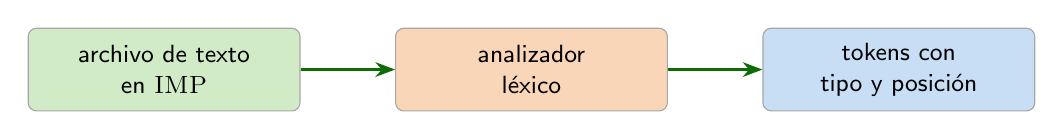
\begin{tikzpicture}[node distance=1.2cm]
\node[bloque,fill=pastelgreen,text width=3.1cm] (a) {archivo de texto\\en \textsc{IMP}};
\node[bloque,fill=pastelpeach,right=of a,text width=3.1cm] (b) {analizador\\léxico};
\node[bloque,fill=pastelblue,right=of b,text width=3.1cm] (c) {tokens con\\tipo y posición};
\draw[arrow] (a) -- (b);
\draw[arrow] (b) -- (c);
\end{tikzpicture}
}
\end{center}

\bigskip

\begin{block}{Pregunta guía}
¿Qué debemos especificar, construir y probar para que la transformación sea reproducible?
\end{block}

\vfill
\end{frame}

\begin{frame}{Producto que construiremos}
\vfill

\begin{columns}[T,onlytextwidth]
\begin{column}{.48\textwidth}
\begin{block}{Código}
\begin{itemize}
  \item AFD de localidades.
  \item Reglas léxicas con \textsc{Lark}.
  \item Tabla inicial de localidades.
  \item Controlador y pruebas.
\end{itemize}
\end{block}
\end{column}
\begin{column}{.48\textwidth}
\begin{block}{Evidencias}
\begin{itemize}
  \item Entradas correctas y errores.
  \item Resultados esperados y reales.
  \item \texttt{README.md} y dependencias.
  \item Historial de \textsc{Git} y reporte.
\end{itemize}
\end{block}
\end{column}
\end{columns}

\bigskip

\begin{center}
\term{El lexer quedará preparado para alimentar al analizador sintáctico.}
\end{center}

\vfill
\end{frame}

\begin{frame}{Ruta de trabajo}
\vfill

\begin{center}
\resizebox{.96\textwidth}{!}{%
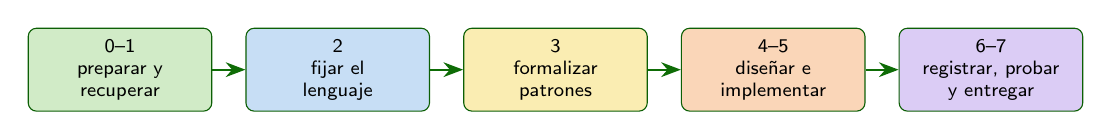
\begin{tikzpicture}[node distance=.42cm]
\node[paso,fill=pastelgreen] (a) {0--1\\preparar y\\recuperar};
\node[paso,fill=pastelblue,right=of a] (b) {2\\fijar el\\lenguaje};
\node[paso,fill=pastelyellow,right=of b] (c) {3\\formalizar\\patrones};
\node[paso,fill=pastelpeach,right=of c] (d) {4--5\\diseñar e\\implementar};
\node[paso,fill=pastelviolet,right=of d] (e) {6--7\\registrar, probar\\y entregar};
\draw[arrow] (a) -- (b);
\draw[arrow] (b) -- (c);
\draw[arrow] (c) -- (d);
\draw[arrow] (d) -- (e);
\end{tikzpicture}%
}
\end{center}

\bigskip

\begin{block}{Ritmo}
Predicción \(\rightarrow\) cambio pequeño \(\rightarrow\) prueba \(\rightarrow\) comparación \(\rightarrow\) evidencia.
\end{block}

\vfill
\end{frame}

\begin{frame}{El compilador como software de sistemas}
\vfill

\begin{columns}[T,onlytextwidth]
\begin{column}{.48\textwidth}
\begin{block}{Conecta representaciones}
Recibe un programa descrito en un lenguaje y produce otra representación que conserva el comportamiento definido.
\end{block}
\end{column}
\begin{column}{.48\textwidth}
\begin{block}{Organiza responsabilidades}
Cada fase recibe información, realiza una tarea delimitada y entrega un resultado a la fase siguiente.
\end{block}
\end{column}
\end{columns}

\bigskip

\begin{center}
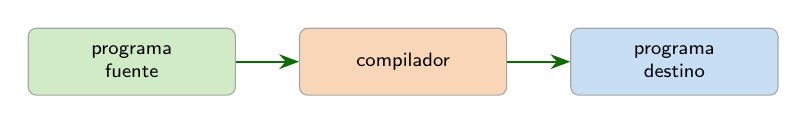
\begin{tikzpicture}[node distance=.8cm]
\node[mini,fill=pastelgreen] (a) {programa\\fuente};
\node[mini,fill=pastelpeach,right=of a] (b) {compilador};
\node[mini,fill=pastelblue,right=of b] (c) {programa\\destino};
\draw[arrow] (a) -- (b);
\draw[arrow] (b) -- (c);
\end{tikzpicture}
\end{center}

\vfill
\end{frame}

\begin{frame}{Abrimos el compilador}
\vfill

\begin{center}
\resizebox{.96\textwidth}{!}{%
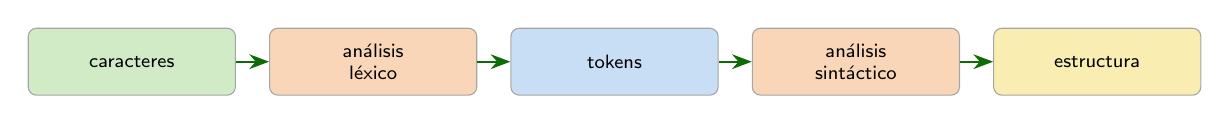
\begin{tikzpicture}[node distance=.42cm]
\node[mini,fill=pastelgreen] (a) {caracteres};
\node[mini,fill=pastelpeach,right=of a] (b) {análisis\\léxico};
\node[mini,fill=pastelblue,right=of b] (c) {tokens};
\node[mini,fill=pastelpeach,right=of c] (d) {análisis\\sintáctico};
\node[mini,fill=pastelyellow,right=of d] (e) {estructura};
\draw[arrow] (a) -- (b);
\draw[arrow] (b) -- (c);
\draw[arrow] (c) -- (d);
\draw[arrow] (d) -- (e);
\end{tikzpicture}%
}
\end{center}

\bigskip

\begin{block}{Foco de la práctica}
Sólo construiremos el tramo caracteres \(\rightarrow\) tokens. No comprobaremos todavía la estructura completa, las declaraciones ni los tipos.
\end{block}

\vfill
\end{frame}

\begin{frame}{Contrato del analizador léxico}
\vfill

\begin{center}
\small
\renewcommand{\arraystretch}{1.35}
\begin{tabular}{|L{.18\textwidth}|L{.66\textwidth}|}
\hline
\textbf{Entrada} & flujo de caracteres del programa fuente \\
\hline
\textbf{Tarea} & agrupar caracteres, reconocer lexemas, clasificarlos y conservar atributos \\
\hline
\textbf{Salida} & secuencia de tokens con información de sus apariciones \\
\hline
\textbf{Consumidor} & analizador sintáctico \\
\hline
\end{tabular}
\end{center}

\bigskip

\begin{alertblock}{Límite}
Reconocer \texttt{X} como localidad no permite decidir si fue declarada, qué tipo tiene o qué valor almacena.
\end{alertblock}

\vfill
\end{frame}

\begin{frame}{Trabajo con la guía práctica}
\vfill
\begin{center}
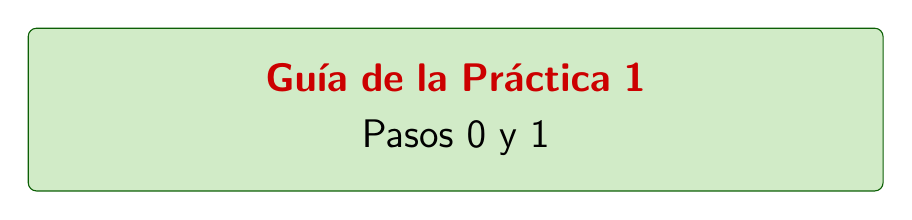
\begin{tikzpicture}
\node[idea,fill=pastelgreen,text width=.82\textwidth,inner sep=13pt,font=\Large]
{\actividad{Guía de la Práctica 1}\\[2pt]Pasos 0 y 1};
\end{tikzpicture}
\end{center}
\bigskip
\begin{itemize}
  \item Ejecutar la versión mínima antes de modificarla.
  \item Completar el recorrido y el contrato léxico.
  \item Comparar el límite de responsabilidad en parejas.
\end{itemize}
\vfill
\end{frame}

\begin{frame}{Función del analizador léxico}
\vfill

\begin{center}
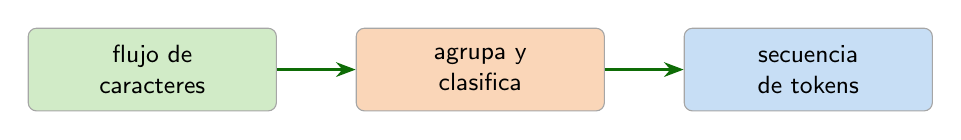
\begin{tikzpicture}[node distance=1cm]
\node[bloque,fill=pastelgreen] (a) {flujo de\\caracteres};
\node[bloque,fill=pastelpeach,right=of a] (b) {agrupa y\\clasifica};
\node[bloque,fill=pastelblue,right=of b] (c) {secuencia\\de tokens};
\draw[arrow] (a) -- (b);
\draw[arrow] (b) -- (c);
\end{tikzpicture}
\end{center}

\bigskip

\begin{itemize}
  \item Puede omitir espacios cuando la convención lo permite.
  \item Conserva información necesaria para fases posteriores.
  \item Informa dónde comienza una unidad o un error.
\end{itemize}

\vfill
\end{frame}

\begin{frame}{Token, lexema, patrón y atributo}
\vfill

\begin{center}
\small
\renewcommand{\arraystretch}{1.35}
\begin{tabular}{|L{.18\textwidth}|L{.68\textwidth}|}
\hline
\textbf{Lexema} & caracteres concretos encontrados, por ejemplo \texttt{X2} \\
\hline
\textbf{Patrón} & forma admitida para un conjunto de lexemas \\
\hline
\textbf{Token} & nombre de categoría que comunica el reconocimiento \\
\hline
\textbf{Atributo} & información de la aparición: texto, valor o posición \\
\hline
\end{tabular}
\end{center}

\bigskip

\begin{block}{Cuatro preguntas}
¿Qué apareció?, ¿qué forma satisface?, ¿qué nombre se emite? y ¿qué información debe conservarse?
\end{block}

\vfill
\end{frame}

\begin{frame}{\textsc{IMP}: conjuntos sintácticos}
\vfill

\begin{center}
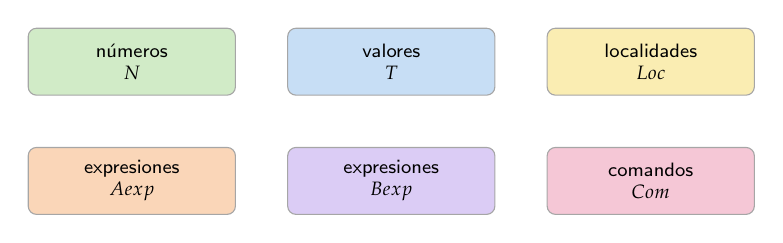
\begin{tikzpicture}[node distance=.65cm]
\node[mini,fill=pastelgreen] (n) {números\\\(N\)};
\node[mini,fill=pastelblue,right=of n] (t) {valores\\\(T\)};
\node[mini,fill=pastelyellow,right=of t] (l) {localidades\\\(Loc\)};
\node[mini,fill=pastelpeach,below=of n] (a) {expresiones\\\(Aexp\)};
\node[mini,fill=pastelviolet,right=of a] (b) {expresiones\\\(Bexp\)};
\node[mini,fill=pastelrose,right=of b] (c) {comandos\\\(Com\)};
\end{tikzpicture}
\end{center}

\bigskip

\begin{block}{Fuente de trabajo}
Winskel presenta \textsc{IMP} como un lenguaje imperativo pequeño con expresiones aritméticas, expresiones booleanas y comandos que modifican un estado.
\end{block}

\vfill
\end{frame}

\begin{frame}{Sintaxis abstracta de \textsc{IMP}}
\vfill

\small
\[
\begin{aligned}
a &::= n \mid X \mid a_0+a_1 \mid a_0-a_1 \mid a_0\times a_1,\\[2pt]
b &::= true \mid false \mid a_0=a_1 \mid a_0\leq a_1
      \mid \neg b \mid b_0\land b_1 \mid b_0\lor b_1,\\[2pt]
c &::= skip \mid X:=a \mid c_0;c_1
      \mid if\ b\ then\ c_0\ else\ c_1
      \mid while\ b\ do\ c.
\end{aligned}
\]

\begin{block}{Qué obtenemos}
Un vocabulario que debe poder escribirse y reconocerse. La sintaxis abstracta no fija por sí sola todas las precedencias ni todos los detalles del texto fuente.
\end{block}

\vfill
\end{frame}

\begin{frame}{Abstracta no significa concreta}
\vfill

\begin{columns}[T,onlytextwidth]
\begin{column}{.48\textwidth}
\begin{block}{Sintaxis abstracta}
Indica cómo se construyen expresiones y comandos. Ayuda a pensar en su estructura.
\end{block}
\end{column}
\begin{column}{.48\textwidth}
\begin{block}{Escritura concreta}
Decide qué caracteres se usan, cómo se agrupa y qué convenciones deberá reconocer el lexer.
\end{block}
\end{column}
\end{columns}

\bigskip

\begin{alertblock}{Decisión visible}
La práctica documentará una convención ASCII. No presentaremos esa adaptación como si fuera una regla literal de Winskel.
\end{alertblock}

\vfill
\end{frame}

\begin{frame}{Convención concreta del curso}
\vfill

\begin{center}
\small
\renewcommand{\arraystretch}{1.28}
\begin{tabular}{|c|c|c|}
\hline
\textbf{Abstracta} & \textbf{Archivo} & \textbf{Token} \\
\hline
\(\times\) & \texttt{*} & \texttt{TIMES} \\
\hline
\(\leq\) & \texttt{<=} & \texttt{LE} \\
\hline
\(\neg,\land,\lor\) & \texttt{!}, \texttt{\&\&}, \texttt{||} & \texttt{NOT}, \texttt{AND}, \texttt{OR} \\
\hline
\(:=\), \(;\) & \texttt{:=}, \texttt{;} & \texttt{ASSIGN}, \texttt{SEMI} \\
\hline
agrupación & \texttt{(}, \texttt{)} & \texttt{LPAR}, \texttt{RPAR} \\
\hline
\end{tabular}
\end{center}

\bigskip

\begin{block}{Numerales}
\texttt{NUM} contiene dígitos; \texttt{-} se emite aparte como \texttt{MINUS}. Así la fase léxica no cambia de decisión según el contexto.
\end{block}

\vfill
\end{frame}

\begin{frame}{Inventario léxico}
\vfill

\begin{center}
\scriptsize
\renewcommand{\arraystretch}{1.25}
\begin{tabular}{|L{.19\textwidth}|L{.68\textwidth}|}
\hline
\textbf{Datos} & \texttt{LOC}, \texttt{NUM} \\
\hline
\textbf{Valores} & \texttt{TRUE}, \texttt{FALSE} \\
\hline
\textbf{Palabras} & \texttt{SKIP}, \texttt{IF}, \texttt{THEN}, \texttt{ELSE}, \texttt{WHILE}, \texttt{DO} \\
\hline
\textbf{Aritmética} & \texttt{PLUS}, \texttt{MINUS}, \texttt{TIMES} \\
\hline
\textbf{Booleanos} & \texttt{EQ}, \texttt{LE}, \texttt{NOT}, \texttt{AND}, \texttt{OR} \\
\hline
\textbf{Control} & \texttt{ASSIGN}, \texttt{SEMI}, \texttt{LPAR}, \texttt{RPAR} \\
\hline
\textbf{Omitido} & espacios, tabuladores y saltos de línea \\
\hline
\end{tabular}
\end{center}

\bigskip

\term{Los nombres formarán parte de la interfaz de la práctica siguiente.}

\vfill
\end{frame}

\begin{frame}{Trabajo con la guía práctica}
\vfill
\begin{center}
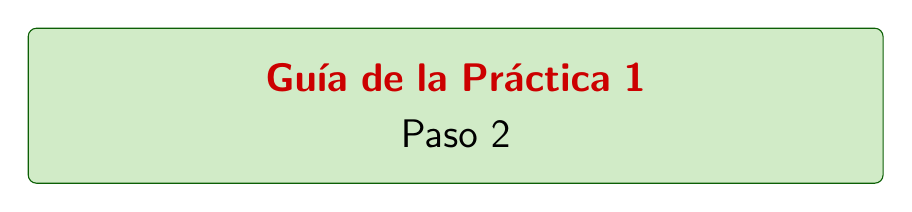
\begin{tikzpicture}
\node[idea,fill=pastelgreen,text width=.82\textwidth,inner sep=13pt,font=\Large]
{\actividad{Guía de la Práctica 1}\\[2pt]Paso 2};
\end{tikzpicture}
\end{center}
\bigskip
\begin{itemize}
  \item Leer la sintaxis abstracta de \textsc{IMP}.
  \item Completar atributos del inventario.
  \item Justificar palabras reservadas, signo y contrato futuro.
\end{itemize}
\vfill
\end{frame}

\begin{frame}{Del patrón a una especificación}
\vfill

\begin{center}
\resizebox{.96\textwidth}{!}{%
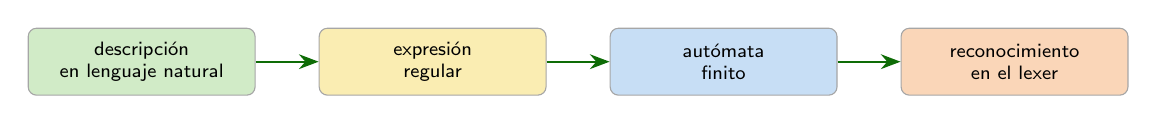
\begin{tikzpicture}[node distance=.8cm]
\node[mini,fill=pastelgreen,text width=2.6cm] (a) {descripción\\en lenguaje natural};
\node[mini,fill=pastelyellow,right=of a,text width=2.6cm] (b) {expresión\\regular};
\node[mini,fill=pastelblue,right=of b,text width=2.6cm] (c) {autómata\\finito};
\node[mini,fill=pastelpeach,right=of c,text width=2.6cm] (d) {reconocimiento\\en el lexer};
\draw[arrow] (a) -- (b);
\draw[arrow] (b) -- (c);
\draw[arrow] (c) -- (d);
\end{tikzpicture}
}
\end{center}

\bigskip

\begin{block}{Dos problemas distintos}
La expresión regular \term{especifica} los lexemas; el autómata \term{reconoce} si una cadena satisface esa forma.
\end{block}

\vfill
\end{frame}

\begin{frame}{Notación que necesitaremos}
\vfill

\begin{center}
\small
\renewcommand{\arraystretch}{1.3}
\begin{tabular}{|c|L{.62\textwidth}|}
\hline
\textbf{Notación} & \textbf{Función} \\
\hline
\texttt{rs} & concatenar una forma seguida de otra \\
\hline
\texttt{r|s} & elegir entre dos formas \\
\hline
\texttt{r*} & repetir cero o más veces \\
\hline
\texttt{r+} & repetir una o más veces \\
\hline
\texttt{r?} & permitir cero o una aparición \\
\hline
\texttt{[A-Za-z]} & elegir un carácter de una clase \\
\hline
\end{tabular}
\end{center}

\bigskip

\begin{alertblock}{Lectura antes de código}
Cada símbolo debe relacionarse con ejemplos que acepta y contraejemplos que rechaza.
\end{alertblock}

\vfill
\end{frame}

\begin{frame}{Modelo: numerales}
\vfill

\begin{center}
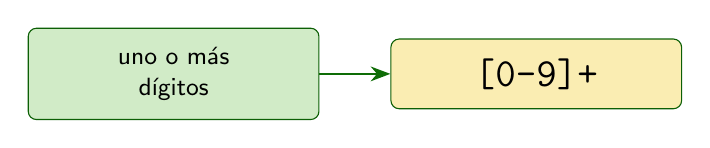
\begin{tikzpicture}[node distance=.9cm]
\node[idea,fill=pastelgreen,text width=3.2cm] (a) {uno o más\\dígitos};
\node[idea,fill=pastelyellow,right=of a,text width=3.2cm,font=\Large] (b) {\texttt{[0-9]+}};
\draw[arrow] (a) -- (b);
\end{tikzpicture}
\end{center}

\bigskip

\begin{center}
\small
\begin{tabular}{|c|c|}
\hline
\textbf{Acepta} & \textbf{Rechaza como un solo \texttt{NUM}} \\
\hline
\texttt{0}, \texttt{25}, \texttt{2026} & cadena vacía, \texttt{X}, \texttt{-3} \\
\hline
\end{tabular}
\end{center}

\bigskip

\term{El signo menos será otro token.}

\vfill
\end{frame}

\begin{frame}{Ahora: localidades}
\vfill

\begin{block}{Descripción}
Una o más letras seguidas opcionalmente por cero o más dígitos.
\end{block}

\bigskip

\[
\texttt{LOC} = \quad \text{\Large ?}
\]

\begin{center}
\small
\begin{tabular}{|c|c|}
\hline
\textbf{Candidatos} & \textbf{Contraejemplos} \\
\hline
\texttt{X}, \texttt{contador}, \texttt{X2}, \texttt{Total25}
&
\texttt{2X}, \texttt{X\_2}, \texttt{X2Y}
\\
\hline
\end{tabular}
\end{center}

\bigskip

\begin{alertblock}{Antes de proponer}
La expresión debe aceptar todos los candidatos y rechazar todos los contraejemplos.
\end{alertblock}

\vfill
\end{frame}

\begin{frame}{Trabajo con la guía práctica}
\vfill
\begin{center}
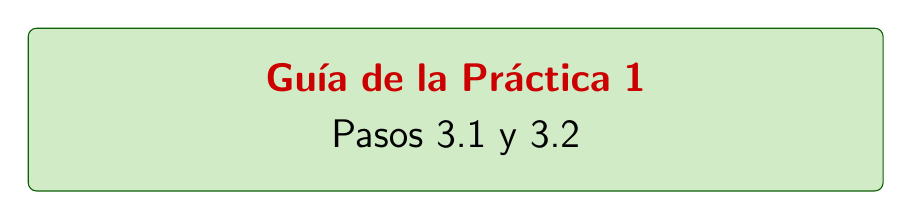
\begin{tikzpicture}
\node[idea,fill=pastelgreen,text width=.82\textwidth,inner sep=13pt,font=\Large]
{\actividad{Guía de la Práctica 1}\\[2pt]Pasos 3.1 y 3.2};
\end{tikzpicture}
\end{center}
\bigskip
\begin{itemize}
  \item Leer la expresión de los numerales.
  \item Derivar el patrón de localidades.
  \item Probar candidatos y contraejemplos antes del AFD.
\end{itemize}
\vfill
\end{frame}

\begin{frame}{Autómata finito determinista}
\vfill

\begin{columns}[T,onlytextwidth]
\begin{column}{.48\textwidth}
\begin{block}{Componentes}
\begin{itemize}
  \item estados;
  \item alfabeto;
  \item transiciones;
  \item estado inicial;
  \item estados finales.
\end{itemize}
\end{block}
\end{column}
\begin{column}{.48\textwidth}
\begin{block}{Funcionamiento}
Consume un símbolo a la vez. Una cadena se acepta cuando se agota la entrada en un estado final.
\end{block}
\end{column}
\end{columns}

\bigskip

\term{Determinista: para cada par estado--símbolo hay como máximo una transición.}

\vfill
\end{frame}

\begin{frame}{Modelo: AFD para \texttt{[0-9]+}}
\vfill

\begin{center}
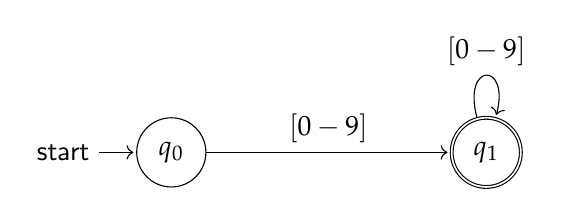
\begin{tikzpicture}[shorten >=1pt,node distance=4cm,on grid,auto]
\node[state,initial] (q0) {\(q_0\)};
\node[state,accepting,right=of q0] (q1) {\(q_1\)};
\path[->]
  (q0) edge node {\([0-9]\)} (q1)
  (q1) edge[loop above] node {\([0-9]\)} (q1);
\end{tikzpicture}
\end{center}

\bigskip

\begin{columns}[T,onlytextwidth]
\begin{column}{.48\textwidth}
\begin{block}{\(q_0\)}
Todavía no se ha leído ningún dígito. No es final.
\end{block}
\end{column}
\begin{column}{.48\textwidth}
\begin{block}{\(q_1\)}
Ya se leyó al menos un dígito. Es final y puede consumir más.
\end{block}
\end{column}
\end{columns}

\vfill
\end{frame}

\begin{frame}{De AFN a AFD y a una versión mínima}
\vfill

\begin{center}
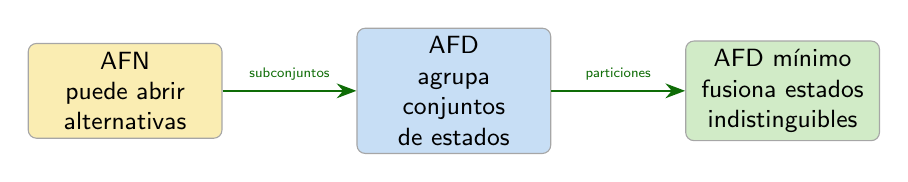
\begin{tikzpicture}[node distance=1.7cm]
\node[bloque,fill=pastelyellow,text width=2.25cm,inner sep=3pt] (a) {AFN\\puede abrir\\alternativas};
\node[bloque,fill=pastelblue,text width=2.25cm,inner sep=3pt,right=of a] (b) {AFD\\agrupa conjuntos\\de estados};
\node[bloque,fill=pastelgreen,text width=2.25cm,inner sep=3pt,right=of b] (c) {AFD mínimo\\fusiona estados\\indistinguibles};
\draw[arrow] (a) -- node[above,font=\tiny]{subconjuntos} (b);
\draw[arrow] (b) -- node[above,font=\tiny]{particiones} (c);
\end{tikzpicture}
\end{center}

\bigskip

\begin{itemize}
  \item El cierre \(\varepsilon\) reúne estados alcanzables sin consumir entrada.
  \item Cada conjunto alcanzable se convierte en un estado determinista.
  \item Se eliminan estados inalcanzables.
  \item Sólo se fusionan estados que no pueden distinguirse con entradas futuras.
\end{itemize}

\vfill
\end{frame}

\begin{frame}{Qué debe recordar el AFD de localidades}
\vfill

\begin{center}
\resizebox{.96\textwidth}{!}{%
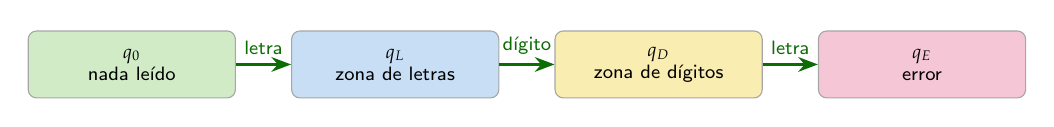
\begin{tikzpicture}[node distance=.7cm]
\node[mini,fill=pastelgreen] (a) {\(q_0\)\\nada leído};
\node[mini,fill=pastelblue,right=of a] (b) {\(q_L\)\\zona de letras};
\node[mini,fill=pastelyellow,right=of b] (c) {\(q_D\)\\zona de dígitos};
\node[mini,fill=pastelrose,right=of c] (d) {\(q_E\)\\error};
\draw[arrow] (a) -- node[above,font=\scriptsize]{letra} (b);
\draw[arrow] (b) -- node[above,font=\scriptsize]{dígito} (c);
\draw[arrow] (c) -- node[above,font=\scriptsize]{letra} (d);
\end{tikzpicture}
}
\end{center}

\bigskip

\begin{block}{Estados finales}
\(q_L\) y \(q_D\) aceptan. No pueden fusionarse: desde \(q_L\) aún se admite otra letra; desde \(q_D\), no.
\end{block}

\begin{alertblock}{Tarea}
Completar todas las transiciones y comprobarlas con candidatos y contraejemplos.
\end{alertblock}

\vfill
\end{frame}

\begin{frame}{Trabajo con la guía práctica}
\vfill
\begin{center}
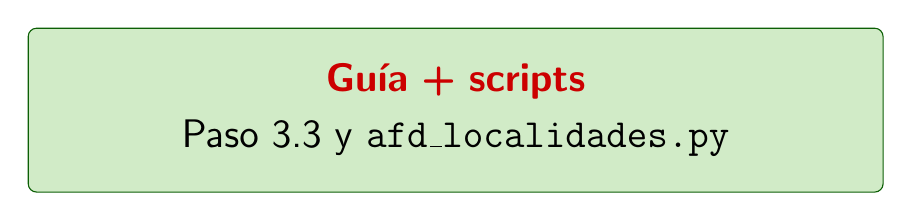
\begin{tikzpicture}
\node[idea,fill=pastelgreen,text width=.82\textwidth,inner sep=13pt,font=\Large]
{\actividad{Guía + scripts}\\[2pt]Paso 3.3 y \texttt{afd\_localidades.py}};
\end{tikzpicture}
\end{center}
\bigskip
\begin{itemize}
  \item Completar la tabla del AFD.
  \item Implementar las transiciones faltantes.
  \item Habilitar las pruebas del paso 3.3.
\end{itemize}
\vfill
\end{frame}

\begin{frame}{Diseñar antes de programar}
\vfill

\begin{center}
\small
\renewcommand{\arraystretch}{1.3}
\begin{tabular}{|L{.18\textwidth}|L{.24\textwidth}|L{.20\textwidth}|L{.22\textwidth}|}
\hline
\textbf{Token} & \textbf{Patrón} & \textbf{Acción} & \textbf{Atributo} \\
\hline
\texttt{LOC} & por completar & emitir y registrar & lexema y posición \\
\hline
\texttt{NUM} & \texttt{[0-9]+} & emitir & lexema o valor \\
\hline
\texttt{IF} & \texttt{"if"} & emitir & no requiere \\
\hline
\texttt{WS} & espacios & omitir & posición actualizada \\
\hline
\end{tabular}
\end{center}

\bigskip

\begin{block}{Contrato ejecutable}
La tabla debe coincidir con la gramática léxica, la salida observada y los resultados esperados de las pruebas.
\end{block}

\vfill
\end{frame}

\begin{frame}[fragile]{Una colisión: \texttt{if} también parece \texttt{LOC}}
\vfill

\begin{center}
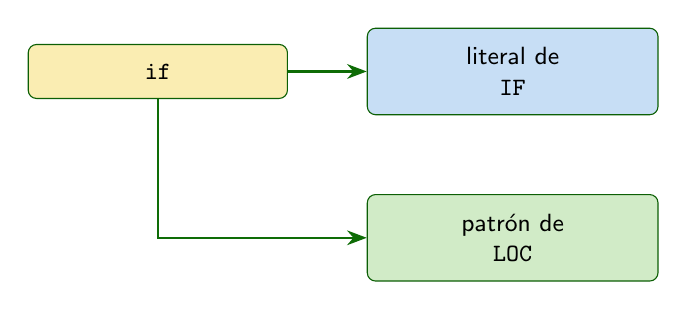
\begin{tikzpicture}[node distance=1cm]
\node[idea,fill=pastelyellow,text width=2.8cm] (a) {\texttt{if}};
\node[idea,fill=pastelblue,right=of a,text width=3.2cm] (b) {literal de\\\texttt{IF}};
\node[idea,fill=pastelgreen,below=of b,text width=3.2cm] (c) {patrón de\\\texttt{LOC}};
\draw[arrow] (a) -- (b);
\draw[arrow] (a) |- (c);
\end{tikzpicture}
\end{center}

\bigskip

\begin{lstlisting}[language={}]
IF.2: /if(?![A-Za-z0-9])/
LOC: /[A-Za-z]+[0-9]*/
\end{lstlisting}

\begin{block}{Decisión}
La prioridad resuelve el empate exacto; el límite evita cortar una localidad más larga. Por eso \texttt{if} es \texttt{IF}, pero \texttt{if2} e \texttt{ifX} son \texttt{LOC}.
\end{block}

\vfill
\end{frame}

\begin{frame}{Trabajo con la guía práctica}
\vfill
\begin{center}
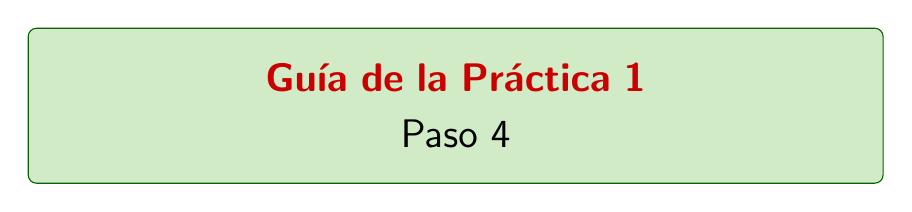
\begin{tikzpicture}
\node[idea,fill=pastelgreen,text width=.82\textwidth,inner sep=13pt,font=\Large]
{\actividad{Guía de la Práctica 1}\\[2pt]Paso 4};
\end{tikzpicture}
\end{center}
\bigskip
\begin{itemize}
  \item Completar la tabla de reglas.
  \item Predecir \texttt{if}, \texttt{if2} e \texttt{ifX}.
  \item Escribir la secuencia esperada antes de modificar el lexer.
\end{itemize}
\vfill
\end{frame}

\begin{frame}{Los scripts siguen la misma ruta}
\vfill

\begin{center}
\resizebox{.96\textwidth}{!}{%
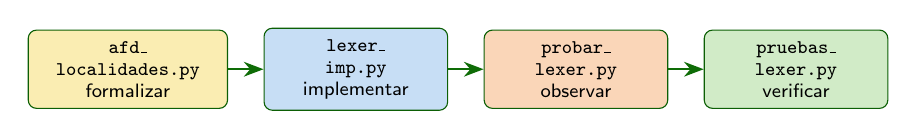
\begin{tikzpicture}[node distance=.45cm]
\node[paso,fill=pastelyellow,text width=2.25cm] (a) {\texttt{afd\_}\\\texttt{localidades.py}\\formalizar};
\node[paso,fill=pastelblue,right=of a] (b) {\texttt{lexer\_}\\\texttt{imp.py}\\implementar};
\node[paso,fill=pastelpeach,right=of b] (c) {\texttt{probar\_}\\\texttt{lexer.py}\\observar};
\node[paso,fill=pastelgreen,right=of c] (d) {\texttt{pruebas\_}\\\texttt{lexer.py}\\verificar};
\draw[arrow] (a) -- (b);
\draw[arrow] (b) -- (c);
\draw[arrow] (c) -- (d);
\end{tikzpicture}%
}
\end{center}

\bigskip

\begin{block}{Punto de partida}
La versión inicial sólo reconoce \texttt{LOC} y omite espacios. Los \texttt{TODO} indican los incrementos; las pruebas se habilitan por paso.
\end{block}

\vfill
\end{frame}

\begin{frame}[fragile]{Lexer mínimo con \textsc{Lark}}
\vfill

\begin{lstlisting}
from lark import Lark

GRAMATICA_LEXICA = r"""
LOC: /[A-Za-z]+[0-9]*/
%import common.WS
%ignore WS
"""

lexer = Lark(
    GRAMATICA_LEXICA,
    parser=None,
    lexer="basic",
)

tokens = list(lexer.lex("X"))
\end{lstlisting}

\begin{block}{Separación de fases}
\texttt{parser=None} y \texttt{lex()} permiten observar el lexer sin introducir todavía una gramática sintáctica.
\end{block}

\vfill
\end{frame}

\begin{frame}{Trabajo con la guía práctica}
\vfill
\begin{center}
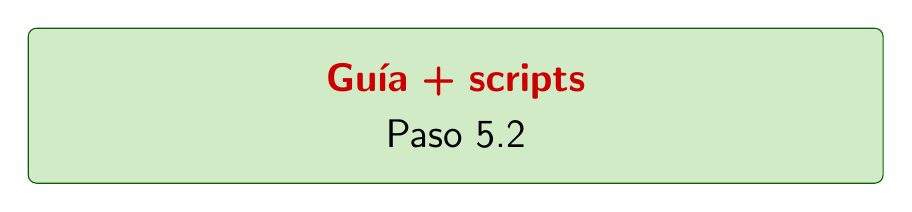
\begin{tikzpicture}
\node[idea,fill=pastelgreen,text width=.82\textwidth,inner sep=13pt,font=\Large]
{\actividad{Guía + scripts}\\[2pt]Paso 5.2};
\end{tikzpicture}
\end{center}
\bigskip
\begin{itemize}
  \item Incorporar \texttt{NUM}.
  \item Habilitar la prueba de localidades y numerales.
  \item Registrar el cambio y su resultado.
\end{itemize}
\vfill
\end{frame}

\begin{frame}{Extender sin perder el control}
\vfill

\begin{center}
\resizebox{.96\textwidth}{!}{%
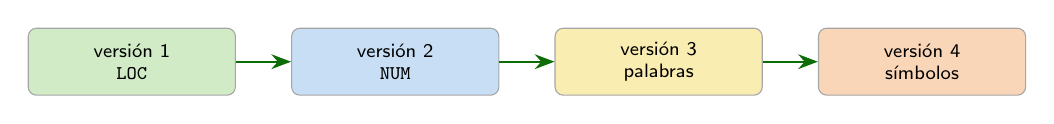
\begin{tikzpicture}[node distance=.7cm]
\node[mini,fill=pastelgreen] (a) {versión 1\\\texttt{LOC}};
\node[mini,fill=pastelblue,right=of a] (b) {versión 2\\\texttt{NUM}};
\node[mini,fill=pastelyellow,right=of b] (c) {versión 3\\palabras};
\node[mini,fill=pastelpeach,right=of c] (d) {versión 4\\símbolos};
\draw[arrow] (a) -- (b);
\draw[arrow] (b) -- (c);
\draw[arrow] (c) -- (d);
\end{tikzpicture}
}
\end{center}

\bigskip

\begin{itemize}
  \item Una nueva categoría se acompaña de su prueba.
  \item Las palabras reservadas se verifican contra \texttt{LOC}.
  \item Los operadores de dos caracteres se prueban completos.
  \item La salida esperada no se ajusta para ocultar un error.
\end{itemize}

\vfill
\end{frame}

\begin{frame}{Trabajo con la guía práctica}
\vfill
\begin{center}
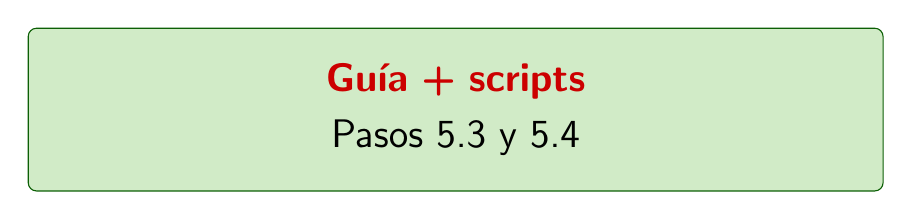
\begin{tikzpicture}
\node[idea,fill=pastelgreen,text width=.82\textwidth,inner sep=13pt,font=\Large]
{\actividad{Guía + scripts}\\[2pt]Pasos 5.3 y 5.4};
\end{tikzpicture}
\end{center}
\bigskip
\begin{itemize}
  \item Incorporar palabras reservadas con prioridad y límite léxico.
  \item Incorporar operadores y delimitadores.
  \item Ejecutar \texttt{flujo.imp} y \texttt{control.imp}.
\end{itemize}
\vfill
\end{frame}

\begin{frame}{Atributos observables}
\vfill

\begin{center}
\small
\renewcommand{\arraystretch}{1.3}
\begin{tabular}{|c|c|c|c|}
\hline
\textbf{Tipo} & \textbf{Lexema} & \textbf{Línea} & \textbf{Columna} \\
\hline
\texttt{LOC} & \texttt{X} & 1 & 1 \\
\hline
\texttt{ASSIGN} & \texttt{:=} & 1 & 3 \\
\hline
\texttt{NUM} & \texttt{2} & 1 & 6 \\
\hline
\end{tabular}
\end{center}

\bigskip

\begin{block}{Mismo nombre, distinta aparición}
Dos tokens \texttt{LOC} comparten categoría, pero pueden conservar lexemas y posiciones diferentes.
\end{block}

\begin{alertblock}{No adelantar semántica}
La fase léxica no asignará tipos ni decidirá si la localidad fue declarada.
\end{alertblock}

\vfill
\end{frame}

\begin{frame}{Tabla inicial de localidades}
\vfill

\begin{center}
\small
\renewcommand{\arraystretch}{1.3}
\begin{tabular}{|c|c|c|}
\hline
\textbf{Lexema} & \textbf{Primera posición} & \textbf{Apariciones} \\
\hline
\texttt{X} & \(1:1\) & 2 \\
\hline
\texttt{Y} & \(1:10\) & 1 \\
\hline
\end{tabular}
\end{center}

\bigskip

\begin{block}{Propósito limitado}
Registrar identidades y ubicaciones útiles. Los tipos, valores y alcances se incorporarán cuando exista información semántica.
\end{block}

\vfill
\end{frame}

\begin{frame}{Trabajo con la guía práctica}
\vfill
\begin{center}
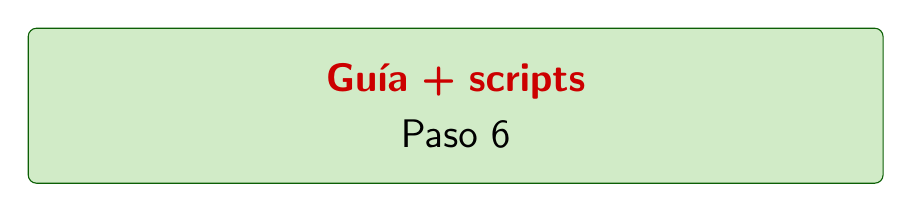
\begin{tikzpicture}
\node[idea,fill=pastelgreen,text width=.82\textwidth,inner sep=13pt,font=\Large]
{\actividad{Guía + scripts}\\[2pt]Paso 6};
\end{tikzpicture}
\end{center}
\bigskip
\begin{itemize}
  \item Observar tipo, lexema, línea y columna.
  \item Completar \texttt{construir\_tabla\_localidades}.
  \item Habilitar la prueba de la tabla.
\end{itemize}
\vfill
\end{frame}

\begin{frame}{Cuando ningún patrón puede avanzar}
\vfill

\begin{center}

\begin{tikzpicture}[node distance=1cm]
\node[idea,fill=pastelgreen,text width=3cm] (a) {\texttt{X := 2}};
\node[idea,fill=pastelrose,right=of a,text width=2cm,font=\Large] (b) {\texttt{@}};
\node[idea,fill=pastelgreen,right=of b,text width=3cm] (c) {\texttt{Y := 3}};
\draw[arrow] (a) -- (b);
\draw[arrow] (b) -- (c);
\end{tikzpicture}
\end{center}

\bigskip

\begin{alertblock}{Error léxico}
\texttt{@} no inicia ninguna categoría aprobada. Informaremos línea y columna y detendremos esta ejecución; no inventaremos una corrección.
\end{alertblock}

\vfill
\end{frame}

\begin{frame}{Matriz mínima de pruebas}
\vfill

\begin{center}
\scriptsize
\renewcommand{\arraystretch}{1.25}
\begin{tabular}{|L{.28\textwidth}|L{.24\textwidth}|L{.30\textwidth}|}
\hline
\textbf{Clase} & \textbf{Ejemplo} & \textbf{Qué comprueba} \\
\hline
Mínimo correcto & \texttt{X} & versión inicial \\
\hline
Varias categorías & \texttt{X := 25;} & segmentación y atributos \\
\hline
Colisión & \texttt{if if2} & prioridad y límite léxico \\
\hline
Operador compuesto & \texttt{<=}, \texttt{:=} & unidad completa \\
\hline
Espacios y líneas & archivo multilinea & omisión y posición \\
\hline
Desconocido & \texttt{@} & diagnóstico léxico \\
\hline
\end{tabular}
\end{center}

\vfill
\end{frame}

\begin{frame}{Trabajo con la guía práctica}
\vfill
\begin{center}
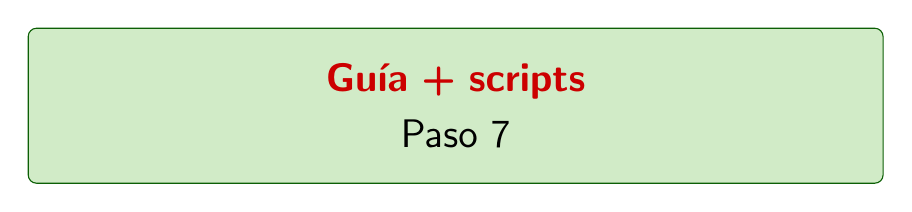
\begin{tikzpicture}
\node[idea,fill=pastelgreen,text width=.82\textwidth,inner sep=13pt,font=\Large]
{\actividad{Guía + scripts}\\[2pt]Paso 7};
\end{tikzpicture}
\end{center}
\bigskip
\begin{itemize}
  \item Ejecutar y explicar el error de \texttt{error.imp}.
  \item Habilitar la última prueba.
  \item Agregar casos propios y preparar evidencias.
\end{itemize}
\vfill
\end{frame}

\begin{frame}{Qué construimos y qué automatiza \textsc{Lark}}
\vfill

\begin{columns}[T,onlytextwidth]
\begin{column}{.48\textwidth}
\begin{block}{Construimos}
\begin{itemize}
  \item categorías y nombres;
  \item patrones y prioridades;
  \item atributos y tabla;
  \item pruebas y diagnósticos.
\end{itemize}
\end{block}
\end{column}
\begin{column}{.48\textwidth}
\begin{block}{\textsc{Lark} apoya}
\begin{itemize}
  \item aplicación de reglas;
  \item recorrido de la entrada;
  \item creación de tokens;
  \item seguimiento de posiciones.
\end{itemize}
\end{block}
\end{column}
\end{columns}

\bigskip

\term{La herramienta ejecuta una especificación; no decide el lenguaje por nosotros.}

\vfill
\end{frame}

\begin{frame}{Antes de entregar}
\vfill

\begin{itemize}
  \item \(\square\) No quedan \texttt{TODO} de la práctica.
  \item \(\square\) Todas las pruebas están habilitadas y pasan.
  \item \(\square\) \texttt{requirements.txt} fija la versión de \textsc{Lark}.
  \item \(\square\) El \texttt{README.md} permite repetir instalación y ejecución.
  \item \(\square\) El reporte contiene decisiones, evidencias, errores y tiempos.
  \item \(\square\) El historial muestra incrementos verificables.
\end{itemize}

\begin{block}{Contrato para continuar}
La lista de nombres de token y sus atributos debe permanecer estable al integrar el parser.
\end{block}

\vfill
\end{frame}

\begin{frame}{Conclusión}
\vfill

\begin{center}
\resizebox{.96\textwidth}{!}{%
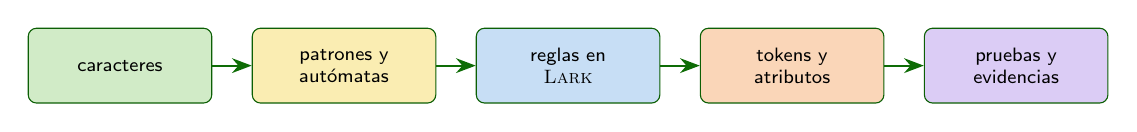
\begin{tikzpicture}[node distance=.5cm]
\node[paso,fill=pastelgreen] (a) {caracteres};
\node[paso,fill=pastelyellow,right=of a] (b) {patrones y\\autómatas};
\node[paso,fill=pastelblue,right=of b] (c) {reglas en\\\textsc{Lark}};
\node[paso,fill=pastelpeach,right=of c] (d) {tokens y\\atributos};
\node[paso,fill=pastelviolet,right=of d] (e) {pruebas y\\evidencias};
\draw[arrow] (a) -- (b);
\draw[arrow] (b) -- (c);
\draw[arrow] (c) -- (d);
\draw[arrow] (d) -- (e);
\end{tikzpicture}%
}
\end{center}

\bigskip

\begin{block}{Idea de cierre}
El lexer materializa el primer contrato interno del compilador. Su corrección depende de especificaciones explícitas, decisiones documentadas y pruebas que hagan visible cada transformación.
\end{block}

\vfill
\end{frame}

\begin{frame}{Referencias}
\vfill
\tiny
\begin{enumerate}
  \item Winskel, G. (1993). \textit{The Formal Semantics of Programming Languages: An Introduction}. The MIT Press.
  \item Aho, A. V., Lam, M. S., Sethi, R., y Ullman, J. D. (2008). \textit{Compiladores: principios, técnicas y herramientas} (2.\textsuperscript{a} ed.). Pearson Educación.
  \item Thain, D. (2026). \textit{Introduction to Compilers and Language Design} (2.\textsuperscript{a} ed.). University of Notre Dame.
  \item Vilar Torres, J. M. (2010). \textit{Estructura de los compiladores e intérpretes}. Universitat Jaume I.
  \item Vilar Torres, J. M. (2010). \textit{Analizador léxico}. Universitat Jaume I.
  \item Lark. (s.\,f.). \textit{API Reference y Grammar Reference}. \url{https://lark-parser.readthedocs.io/}
\end{enumerate}
\vfill
\end{frame}

\end{document}
